\documentclass[english]{article}
\usepackage[utf8]{inputenc}
\usepackage{multicol}
\usepackage{graphicx}
\usepackage[letterpaper, margin=0.85in]{geometry}
\usepackage{blindtext}
\usepackage{caption}
\usepackage{sectsty}
\usepackage{hyperref}
\usepackage{setspace}
\usepackage{pgfplotstable,tabularx,booktabs}
\usepackage{csvsimple}
\usepackage{amsmath}
\usepackage{babel}

\usepackage{mathptmx}% http://ctan.org/pkg/mathptmx
\setlength{\columnsep}{0.3in}

\usepackage{csvsimple} % For csv importing.

\makeatletter
\csvset{
  autotabularcenter/.style={
    file=#1,
    after head=\csv@pretable\begin{tabular}{|*{\csv@columncount}{c|}}\csv@tablehead,
    table head=\hline\csvlinetotablerow\\\hline,
    late after line=\\,
    table foot=\\\hline,
    late after last line=\csv@tablefoot\end{tabular}\csv@posttable,
    command=\csvlinetotablerow},
  autobooktabularcenter/.style={
    file=#1,
    after head=\csv@pretable\begin{tabular}{*{\csv@columncount}{c}}\csv@tablehead,
    table head=\toprule\csvlinetotablerow\\\midrule,
    late after line=\\,
    table foot=\\\bottomrule,
    late after last line=\csv@tablefoot\end{tabular}\csv@posttable,
    command=\csvlinetotablerow},
}
\makeatother
\newcommand{\csvautotabularcenter}[2][]{\csvloop{autotabularcenter={#2},#1}}
\newcommand{\csvautobooktabularcenter}[2][]{\csvloop{autobooktabularcenter={#2},#1}}

\title{Parallel Acceleration of EpicFlow with Red/Black Successive Over Relaxation Using GPUs with CUDA}
\author{
  Amogh Param\\
  704434779\\
  \texttt{aparam@cs.ucla.edu}
}
\date{June 2016}

\begin{document}
    \maketitle
     
	\section*{Abstract}  
	We propose a parallelization of optical-flow estimation that exploits the ability of Graphical Processing Units (GPU) to process multiple image pixels in parallel to speed up the estimation, under the CUDA environment. The optical flow estimation method involves an energy minimization phase which we solve using an efficient and parallel numerical approximation scheme, Successive Over Relaxation with red-black ordering (Red-Black SOR). In addition, we show that choosing optimal memory  access patterns and allocation strategies are critical in maximizing the speed of computation for the flow estimation. The primary contribution of this project extends EpicFlow\cite{1}, the state-of-the-art in variational optical flow estimation, by replacing the serial optimization procedure with a parallel one deployed on the GPU in the CUDA environment. The same GPU parallelization principles can be used for other flow estimation methods that solve a large optimization problem over pixel values, where the optimization is complex but decomposed into solving a sequence of linear systems of equations with SOR. Our work is focused on data parallelism and threads deployment tuning; the management of which is critical to efficient GPU implementations. Experimental results are shown on NVIDIA GTX 750M and compared against the performance of an Intel Core i7 CPU for image sequences from the Middlebury dataset. The speed-up factor for our set of GPU optimizations reaches 2.5x for successive over relaxation computation time and 2x for the overall execution time for energy minimization as compared to the CPU.\footnote{\href{https://github.com/jazzthejackrabbit/epic-flow-cuda}{github.com/jazzthejackrabbit/epic-flow-cuda}}

    \section{Introduction}
	Programmable GPUs provide a competitive alternative to traditional CPUs by delivering high performance computing with extremely high floating point performance for computer vision and image processing applications \cite{6}. Since the input data in such applications are multidimensional arrays, there has been plenty of research interest in exploiting GPU horsepower for such problems. This is especially true in applications that involve numerical computing techniques. Multidimensional arrays are used as primary data structures in many numerical computing techniques. This provides an opportunity to take advantage of Single Instruction Multiple Data (SIMD) parallelism. However, it is quite challenging to parallelize such techniques for the GPU since most numerical computing techniques are iterative in nature. One such problem of interest in computer vision is the estimation of optical flow.\newline

	Optical flow is a classic computer vision problem where the primary goal is to track moving objects, surfaces and edges in a sequence of image frames by way of computing the displacement of pixels between every pair of frames in the sequence. To achieve this goal, we assume that the gray values of corresponding pixels are the same in both image frames of the pair. Optical flow is important to providing visual systems the ability to discern possibilities for action within an environment \cite{8}. In addition, optical flow stimulus is important for the perception of movement by an observer in the environment; perception of the shape, distance and movement of objects in the environment; and for locomotive control \cite{9}. As a result, it is used as a fundamental framework for applications such as image and surface reconstruction; object tracking and detection; and robot navigation. Animals in the wild make decisions on whether to attack or flee based on visual stimulus derived from the motion of predators or prey. It is paramount that they make such decisions almost instantaneously to save their own lives or to ensure a successful hunt. This provides motivation for building optical flow estimation techniques that are fast and in real time, since optical flow provides vision systems a fundamental way to discern motion.

	\begin{center}
	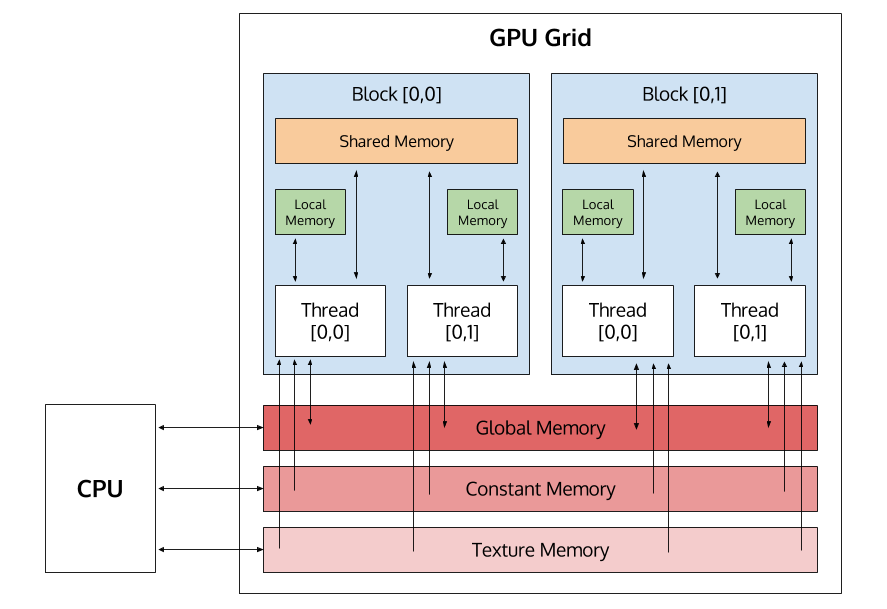
\includegraphics[width=160mm]{results/images/1_gpu_grid.png}
	\captionof{figure}{GPU Architecture and Structure of Communication. 1) Global, Constant and Texture Memory are shared by all the threads. 2) Every thread block shares a common 'shared memory' among its threads. 3) Every thread has access to its own local memory that is not visible to the other threads.}
	\end{center}

	There have been an abundance of optical flow estimation techniques, but it is challenging to deal with occlusions, motion discontinuities and large displacements. Our work extends EpicFlow \cite{1}, an optical flow estimation method that is suitable for large displacements with significant occlusions. EpicFlow's performance is bottlenecked by the process of linearization (warping) and the process of finding solutions to the resulting linear systems of equations by the Successive Over Relaxation (SOR) method. Therefore, in the same spirit as \cite{2}, we use a multi-colored ordering technique for the SOR method to decrease the computational time for optical flow estimation. In addition, accelerating algorithms on the GPU within the CUDA environment can be challenging as the it offers high flexibility in terms of the potential memory types and access strategies that can be used. Therefore, we explore the trade-offs involved in using different GPU based memory access patterns and memory types. It is very important to follow optimal access patterns to get maximum memory bandwidth; especially given how costly accesses to device memory are, thus making it a non-trivial task.\newline

	The rest of the paper is organised as follows: \textbf{Section 2} describes the GPU programming model and architecture. \textbf{Section 3} details the EpicFlow algorithm and explores the parallel variation on energy minimization. \textbf{Section 4} describes the implementational details and experiments for different memory techniques used to improve speed of computation. \textbf{Section 5} presents results and performance benchmarks of the GPU experiments. \textbf{Section 6} provides concluding remarks.
    
	\section{Graphical Processing Unit}
	Graphical Processing Units (GPU), have evolved into highly parallel, multithreaded, multi-core co-processors. They offer more computational horsepower, in comparison to CPUs, by featuring thousands of Arithmetic Logic Units (ALU), hundreds of processors and tens of thousands of concurrent threads per application. GPUs also provide more power efficient hardware for computation. However, it offers a more restrictive programming model and as a result implementations of algorithms on the GPU can be challenging.

	\subsection{CUDA Programming Model and Architecture}
	NVIDIA’s Compute Unified Device Architecture (CUDA), is a general purpose programming model for GPUs. It is a heterogeneous model in which both the CPU and the GPU are used. CUDA refers to the CPU and its memory as the 'host', and to the GPU and its memory as the 'device'. A typical parallel GPU based program involves allocating memory on the device, moving data from the host memory into the allocated device memory, launching and executing computational units (kernels) in parallel by GPU threads and then copying data back into the host from the device. CUDA executes a kernel as a grid of thread-blocks. This allows the computational work to be divided among the available compute resources. Threads in a block share access to a fast memory store independent to each thread-block called shared memory. GPUs feature streaming multiprocessors (SM) which in turn comprise of many simple processors. Multiple thread blocks are assigned to a single SM and all threads in a thread block typically run in lock-step to solve a smaller subproblem. During execution there is a finer grouping of threads into warps. Multiprocessors on the GPU execute instructions for each warp in SIMD (Single Instruction Multiple Data) fashion. \textbf{Figure 1} shows the architecture and structure of communication between the CPU, GPU and the different memory types available on the GPU.

	\section{Optical Flow Estimation}
	\subsection{Edge Preserving Interpolation of Correspondences}
	Edge Preserving Interpolation of Correspondences (EpicFlow) \cite{1} is a novel approach for optical flow estimation, targeted at large displacements with significant occlusions. It consists of a novel scheme to interpolate a sparse set of matches obtained from \cite{3} into a dense correspondence field based on an edge-aware distance instead of Euclidean distance. The distance between matches used in the interpolation is computed based on a cost map derived from \cite{4} which respects motion boundaries. In this way, the distance between pixels belonging to the same region is low and ensures a proper edge-respecting interpolation. The interpolation process initiates the optical flow estimation.

	\subsection{Variational Energy Minimization}
	The dense matches obtained from the interpolation are then used in a variational energy minimization framework. The energy functional is defined as the sum of a data term and a smoothness term. The data term is based on the classical color-constancy and gradient constancy assumption with a normalization factor \cite{5}. The flow gradient norm is penalized with a local smoothness weight for the smoothness term. The output from the sparse-to-dense interpolation is used to initialize the solution of the flow estimate for the energy minimization. The optimization problem is solved by an iterative method that linearizes the objective cost around the current estimate of the flow and estimates a small flow step in the direction of the minimum. This estimation reduces to solving a linear system of equations by successive over relaxation (SOR).

	% The flow updates are then computed by solving linear systems using the successive over relaxation method.

	\subsubsection{Successive Over Relaxation (SOR)}
	The successive over relaxation (SOR) iterative method \cite{10} is an important solver for linear systems. It is widely used to solve linear systems or partial differential equations (PDE) discretized by a finite difference method. It is also very popular in PDE evolution because the characteristics of gradient operators lead to matrices with a structure well suited to SOR. Since it is inherently sequential in its original form, there have been many parallel versions of the SOR method that have been proposed, to take advantage of the tremendously fast computational resources available.\newline 
	
	The energy function is highly nonlinear and a minimizer of such a function must fulfill the Euler-Lagrange equations \cite{13}. The resulting sparse linear system of equations can now be solved by SOR. For matrix A of the linear system Ax = b, the SOR update is:

	\begin{center}
	$x_i^{(k+1)} = (1 - \omega)x_i^{(k)} + \frac{\omega}{a_{ii}}[b_i - \displaystyle\sum_{j=1}^{i-1} a_{ij} x_j^{(k+1)} - \displaystyle\sum_{j=i}^{n} a_{ij}x_j^{(k)}]$
	\end{center}	

	\subsubsection{Red Black Successive Over Relaxation (RB-SOR)}
	A is a sparse pentadiagonal matrix and given this form, there are only 2 values in the above sum that are non zero. These correspond to the left and top neighbors of each pixel. \newline 

	\begin{center}
	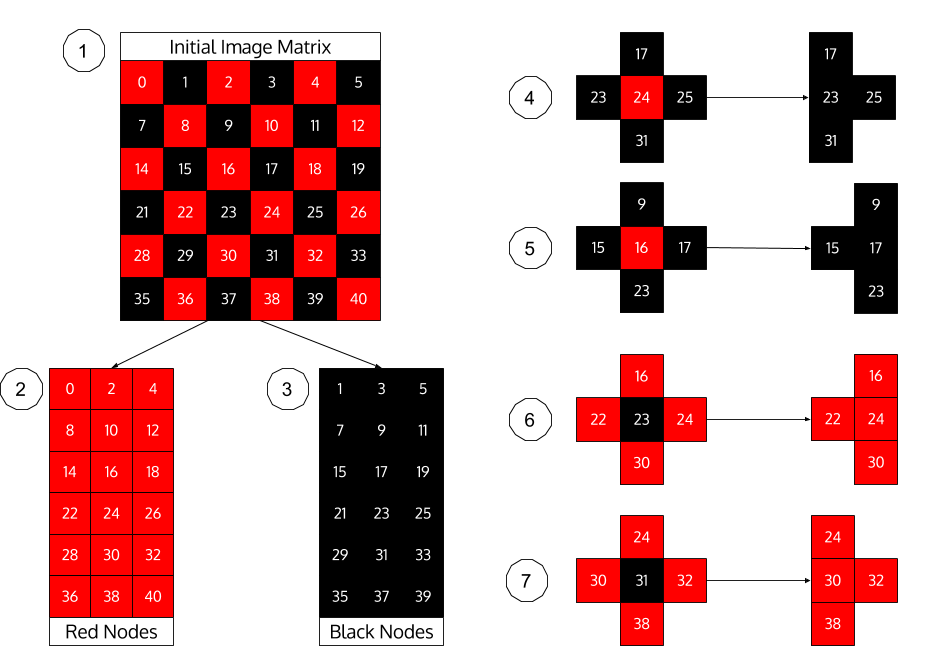
\includegraphics[width=175mm]{results/images/5-rb_order.png}
	\captionof{figure}{(1) Red black ordering of initial image matrix. (2) Matrix of red nodes. (3) Matrix of black nodes. (4-5) Black neighborhood around red nodes (6-7) Red neighborhood around black nodes.}
	\end{center}	

	The first summation depends on updated values of the left and top neighbors from the previous iteration and the second summation depends on values of the right and bottom nieghbors from the same iteration. Due to this and given the form of A, we can split the matrix into a checkerboard pattern of 'red' and 'black' pixels, which are then processed in a color-wise manner. An element at position \textbf{(i, j)} is colored red if \textbf{(i + j)} is even, black if it is odd. The red-black ordering is illustrated in \textbf{Figure 2.1}. The computation of the flow increments takes place in two phases. In the first phase all the red nodes are computed as the flow-update value at each red node only depends on the neighborhood of black nodes \textbf{(Figure 2.4, 2.5)}, which are completely available for all the red nodes. As a result, all the flow increments at red nodes can be partitioned into a number of independent tasks dependent only on their local neighborhood of black nodes and computed in parallel without any dependence on other red nodes. Similarly, in the second phase, the black nodes can be partitioned into independent tasks and computed in parallel as the flow-update values at these nodes only depend on the new values of the local neighborhood of red nodes which are completely available after the first phase \textbf{(Figure 2.6, 2.7)}. %The $\boldsymbol{\omega}$ is the relaxation factor which governs the rate of convergence. Since the primary focus of this paper is the GPU optimizations using this technique, we use the same $\boldsymbol{\omega}$ values as in \cite{1}.\newline

	\section{Implementations and Experiments}
	In this section, we look into various implementation strategies to speed up the process of optical flow estimation. The red-black ordering variation of the successive over relaxation method provides inherent parallelism. There are many factors that could potentially affect the eventual speed-up that can be obtained; including coalesced access to memory, usage of faster memory types available on the GPU, data reordering for efficient access, usage of efficient memory allocation strategies and tuning the configuration of thread blocks deployed on the streaming multiprocessors. Adhering to these access patterns is a requirement for any performant kernel on the GPU. A more comprehensive and detailed description is provided in the CUDA programming guide \cite{11} 

	\begin{center}
	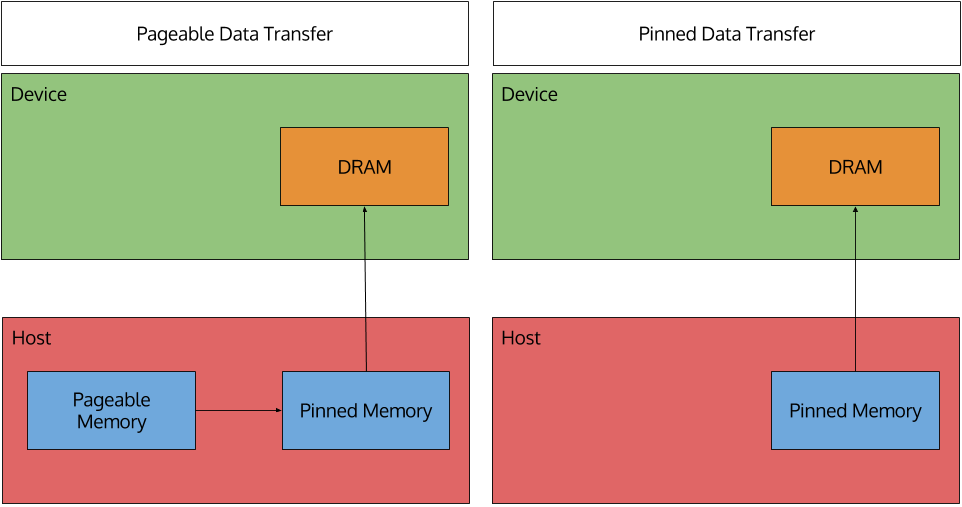
\includegraphics[width=120mm]{results/images/2_pinned_paged.png}
	\captionof{figure}{Pinned v/s Paged Memory Allocation. 1) Pageable Data transfer has the overhead of copying data from pageable memory to pinned memory and then to the GPU. 2) Pinned Data Transfer directly allocates memory on the pinned memory and then transfers to the GPU}
	\end{center}		

	\subsection{Global Memory}
	Using only the global memory provides a simple approach to parallelize any computation that is independent per pixel, specifically the energy minimization. We first copy image data from the CPU (host) memory into the GPU (device) memory. We then define a separate GPU kernel for each of the two colors in the red-black ordering, where each kernel computes the flow update for the successive iteration for nodes of a single color. The kernel for the red nodes is executed first, followed by the kernel for the black nodes. The entire process is done five times to compute the non-linear weights that appear when applying the Euler Lagrange equations and the red-black kernels are executed thirty times to solve the linear systems to obtain the flow updates. 

	\subsubsection{Comparison of Pinned and Paged Memory}
	By default, allocated memory on the host (CPU) is pageable. The device (GPU) cannot access this data from the pageable host memory. As a result, when a data transfer between the CPU and GPU is requested, the CUDA driver first creates a temporary page-locked host array, also known as “pinned” memory. The data is then transferred from the pageable memory to the pinned memory before it is transferred to the device memory (\textbf{Figure 3}).\newline

	Pinned memory is essentially used as a staging area for data transfers between the device and the host. An optimization strategy to improve the data transfer efficiency is to avoid the cost of the transfer between pageable and pinned host arrays by directly allocating our host arrays in pinned memory. We do so by using the CUDA specific API for allocating pinned host memory using cudaMallocHost() or cudaHostAlloc(), and deallocate it with cudaFreeHost(). However, over-allocating pinned memory can reduce overall system performance because it reduces the amount of physical memory available to the operating system and other programs. \textbf{Table 1} shows a comparison between the two allocation strategies.\newline

	Although using pinned host memory directly instead of pageable host memory improves access efficiency and decreases the computational time for the variational energy minimization, we can achieve a greater improvement by using better memory access strategies and faster types of memory.

	\subsubsection{Texture Memory}
	The successive over relaxation method accesses neighbors of a pixel, in a stencil pattern. As a result, such an access pattern doesn’t take advantage of the efficiencies provided by the GPU for coalesced memory access. Texture memory provides an efficient access pattern for the global memory as it features an intermediate memory cache which is optimized for two dimensional locality. A memory segment allocated on the global memory has to be bound to the texture memory using cudaBindTexture() (costless operation) and can then be accessed using efficient read functions such as tex1D(), tex2D() or tex3D(). The texture memory space resides in device memory and is cached in texture cache, so a texture fetch costs one memory read from device memory only on a cache miss, otherwise it just costs one read from texture cache. 

	Since texture cache is optimised for 2D spatial locality, threads of the same 
	 that read texture addresses that are close together in 2D will achieve best performance. Using the texture memory access pattern, we can expect the read access to be much faster than that with global memory not bounded to a texture. Texture memory is a read-only memory and thus provides a speed bump only with respect to read access. All the writes are still performed to the global memory and thus are not at maximum efficiency. 

	\subsection{Coalesced memory access}
	Every time a GPU thread accesses memory, it accesses a larger chunk of memory in one memory transaction. If other threads do the same, then similarly large chunks are accessed for each thread. However, if the other threads access memory contiguously, a new memory transaction is not required for every thread access as a larger chunk of memory is already retrieved by the previous memory transactions. As a result, maximizing coalesced access to memory will speed up the memory reads by the threads, as separate memory transactions will not be required and will allow the GPU program to complete faster. However, in the case of red black SOR, coalescing the access to memory is not as straightforward because the method involves reading elements in a strided pattern (alternate red elements or alternate black elements). Furthermore, it involves reading from the neighbors of an element, access to which is not coalesced or cached.

	\subsubsection{Memory Reorganization}
	In each iteration of the energy minimization, the black and red nodes are accessed first, and then the red nodes are written back, followed by accessing the red and black nodes and writing back the black nodes. This requires a strided pattern of reads and since such a pattern is not contiguous, it decreases the maximum amount of useable memory locations that can be retrieved with each memory transaction. As a result, there are more memory transactions involved. In order to avoid such sparse element accesses and to improve the coalescing, we explore the idea of reordering the elements of the image by grouping elements of the same color into a single matrix \cite{2}.\newline

	We divide the image matrix into two independent single-colored matrices, where one of them comprises only of red colored elements, and the other of only black colored elements (\textbf{Figure 2.2, 2.3}). This reordering is done parallely in the GPU by copying the elements in the original red-black image matrix at position \textbf{(i, j)} to position \textbf{(i/2, j)} in the independent single-colored matrices appropriately, depending on the color of the element. Reordering in such a way allows contiguous access to memory and as a result, warp threads can function at maximum efficiency and increases coalesced access to memory. The red black SOR procedure involves access to black colored neighbor nodes of a red node and similarly red colored neighbor nodes of a black node. Due to the reordering, access to this neighborhood is more complex (\textbf{Figure 2.4 - 2.7}). The neighbors of a red node are three vertical nodes plus one on the left or right, depending on the row number in the reordered matrix of black nodes and vice versa for the neighbors of a black node.

	\subsection{Thread Divergence and Alternate Indexing}
	Threads from a block are bundled into fixed-size warps for execution on a CUDA core, and threads within a warp must follow the same execution trajectory. All threads must execute the same instruction at the same time. In other words, threads cannot diverge. Conditional branching constructs within CUDA kernels can cause thread divergence. Since CUDA has a requirement to have non-divergent warps, having divergent warps has negative performance consequences as the divergent warps are executed serially, instead of in parallel.\newline

	The deployed threads and blocks have indices that can be used to index elements in memory, within the CUDA kernels. These indices are linear and as a result, using the same linear indexing scheme to access alternating red elements in the first kernel and black elements in the second kernel requires a conditional branch, which would result in half the threads in each kernel diverging and hence, ceasing to do any useful computation. Minimizing thread divergence is important to maximize parallel computation on the GPU. As a result, we introduce an efficient alternate indexing scheme which computes the correct index of red elements and black elements within their respective kernels without conditional branching.\newline

	\begin{center}	
	$i_{ra} = 2i + (2(i_t/w) \bmod 2)$
	\end{center}

	\begin{center}	
	$i_{ba} = (2i+1) - (2(i_t/w) \bmod 2)$
	\end{center}

	\begin{center}
	
\includegraphics[width=170mm]{results/images/3_cpu_gpu_gt.png}
	\captionof{figure}{Optical flow estimates from GPU and CPU implementations, and original ground truth optical flow.}
	\end{center}
	
	 $i_{ra}$ is the alternate index for the red nodes in the matrix of red elements, $i_{ba}$ is the alternate index for the black nodes in the matrix of black elements, $i_t$ is the linear thread index, $w$ is the width of the image. Using this indexing scheme, we minimize the divergence of threads and hence increase the computational efficiency.

	\section{Performance Results and Benchmarks}
	We use the NVIDIA GTX 750M GPU for all our experiments and compare the performance of the optical flow estimation against that of an Intel Core i7 CPU. To show that our GPU implementation provides an improvement over the CPU version of EpicFlow, we first show that the average endpoint error in optical flow estimation is the same in CPU and GPU based estimations. Then a comparison is made for computational performance between the CPU implementation and the GPU implementations. We then see how tuning the configuration of threads in a block affects computation time.

	\subsection{Optical Flow Estimation}
	\textbf{Figure 4} shows the optical flow visualized from the output of the GPU implementation, the CPU implementation and the ground truth flow for a sample sequence (Rubber Whale) in the Middlebury dataset \cite{12}. \textbf{Table 1} shows the average endpoint error for the optical flow estimation using the CPU implementations and the GPU implementations.
	
	\begin{center}
	\centering
	\csvautotabularcenter{results/tables/1_aee.csv}	
	\captionof{table}{Average End Point Errors of Optical Flow Estimation}
	\end{center}

	All the GPU implementations have the same average endpoint error as the CPU implementations. As a result, the GPU implementation provides accurate optical flow estimation based on EpicFlow and thus can be used as a viable alternative to the CPU implementation. The following subsections show the improvement of the GPU over the CPU in terms of computational speed.	

	\subsection{Computation and Execution Time}
	The first optimization for global memory access was to allocate data directly on the pinned memory, instead of pageable host memory. \textbf{Table 2} shows that allocating and accessing pinned memory is faster than that of pageable host memory, although it provides only a small speedup.

	\begin{center}
	\csvautotabularcenter{results/tables/2_pinned_paged.csv}	
	\captionof{table}{Execution Time for Pinned v/s Paged Memory Allocation}
	\end{center}

	\begin{center}
	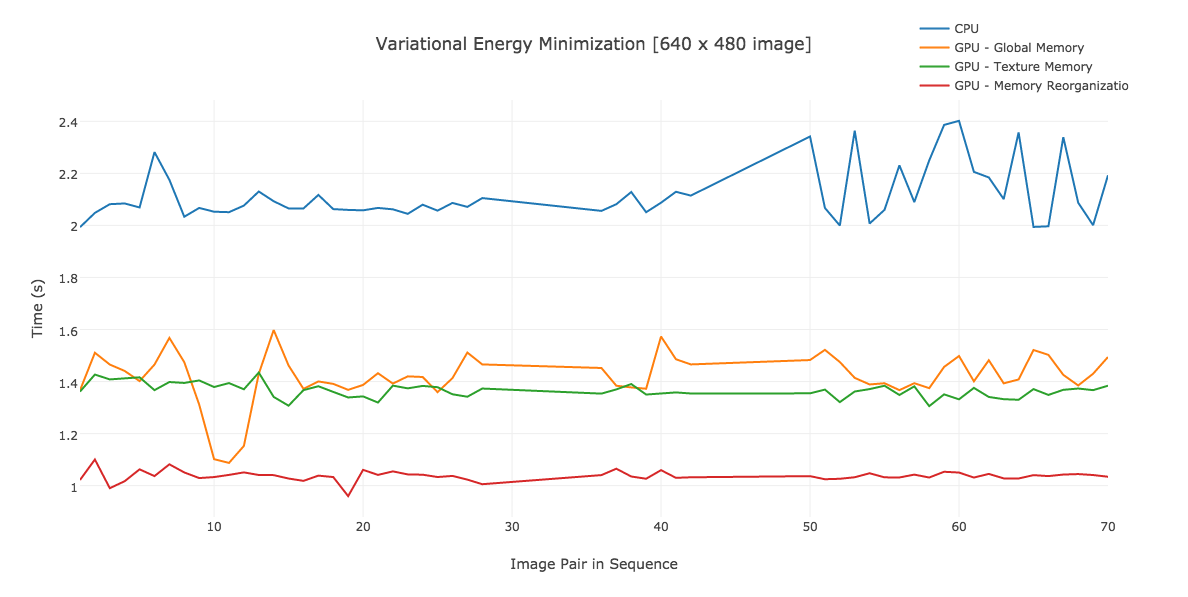
\includegraphics[width=130mm]{results/images/4_1_gpu_cpu_time_comparison.png}
	\captionof{figure}{Execution Time for GPU and CPU implementations.}
	\end{center}

	\begin{center}
	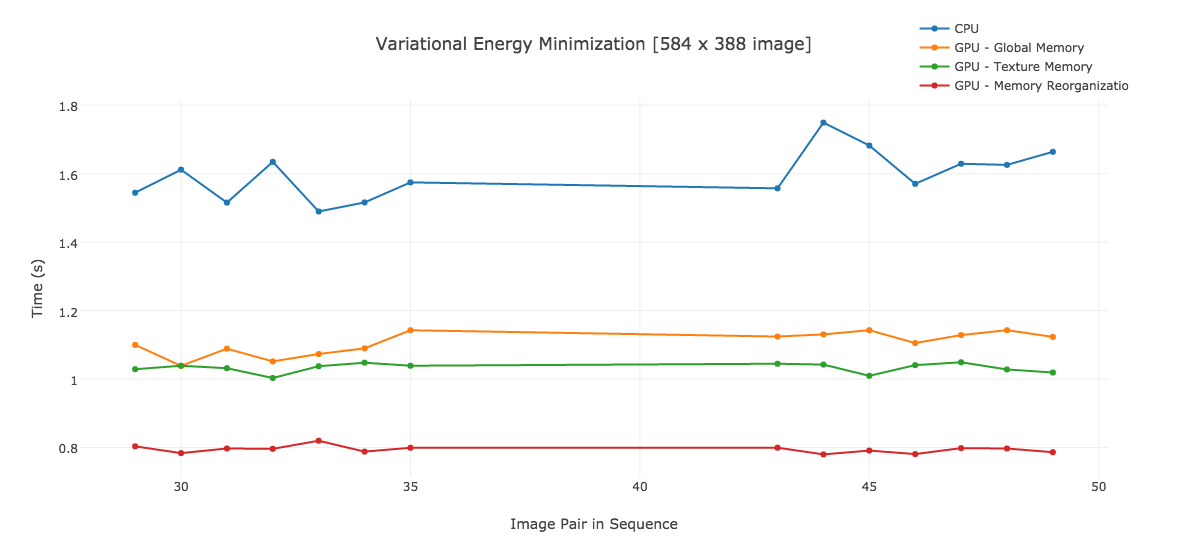
\includegraphics[width=130mm]{results/images/4_2_gpu_cpu_time_comparison.png}
	\captionof{figure}{Execution Time for GPU and CPU implementations.}
	\end{center}


	\textbf{Figure 5} shows the execution time for every pair of image in different sequences in the Middlebury dataset of resolution 640x480, \textbf{Figure 6} shows the same for images of resolution 584x388. \textbf{Table 3} shows the total execution time for the entire energy minimization process and computation time for the SOR method (RB-SOR for GPU), averaged for the images in the Middlebury dataset. As expected, all the GPU implementations perform faster than the CPU implementation. Specifically, the reordering of elements of the same color into two separate matrices performs (on average) 2x faster than the CPU benchmark for total execution time and 2.55x faster in terms of computation time. This indicates that memory coalescing is critical in improving the speed of execution and computation. Global memory with no other optimization is the slowest among the GPU implementations. Although it is 1.48x and 1.8x faster in terms of execution time and computation time respectively, direct global memory access seems to be the bottleneck. Texture memory access pattern provides caching of local neighborhood access and provides a 1.54x and 1.82x improvement in execution and computation time respectively, over the CPU implementation. However, it surprisingly doesn’t provide a huge improvement over direct global memory access. This is most likely because we use a one-dimensional texture. We believe that replacing one dimensional textures with two dimensional textures would improve caching of neighborhood elements and as a result improve the speed of computation.

	\begin{center}
	\csvautotabularcenter{results/tables/3_compute_time.csv}	
	\captionof{table}{Execution Time for CPU and GPU implementations}
	\end{center}

	The speed gain achieved in the computation time is  higher than that of execution time primarily because the execution time takes into consideration the entire process of estimating the flow from the interpolation of dense matches and the computation time only considers the time taken by the SOR method/ Red-black SOR method. Clearly, the raw computational power of the GPU performs better than the serial CPU implementation of SOR (as evident from the computation time), but since the GPU implementation involves allocating memory on the GPU, transferring data between CPU memory and GPU memory, computing flow updates and writing them back to the CPU memory, it creates a bottleneck in terms of read-write memory bandwidth. \textbf{Table 4} shows an example of profiling results obtained by running the parallel implementation of SOR on the GPU, using only global memory. 58.16\% of the execution time is taken up by the memory copy operation to transfer data between the CPU memory and GPU memory. As a result, the maximum optimization for this application is limited by the maximum memory bandwidth.

	\begin{center}
	\csvautotabularcenter{results/tables/4_profile.csv}
	\captionof{table}{GPU Implementation Profiling. The largest chunk of time is taken for the memcpy between HtoD (Host to Device)}
	\end{center}

	Furthermore, the alternate indexing scheme used to address memory locations is important while considering the speed of the computation. \textbf{Table 5} shows a comparison of the time profiles of the two indexing schemes. Using conditional branch within the kernels to choose between the red and black elements is slower than using the alternate indexing scheme that allows access to only red or only black elements within a specific kernel. The alternate indexing provides an average of 1.14x speedup in execution time as compared to the conditional indexing.

	\begin{center}
	\csvautotabularcenter{results/tables/5_alternate_index.csv}
	\captionof{table}{Kernel Execution time for indexing schemes}
	\end{center}

	\subsection{Thread Configuration}
	\textbf{Table 6} shows the execution times for different configurations of the best performing (memory reorganized) GPU implementation. It performs best with a 16x8 (128) threads in a block configuration, with an execution time of 965.2 ms. The best thread configuration will be different on other GPUs as it is a factor dependent on the specific hardware limitations of the GPU.	The NVIDIA architecture deploys blocks based on the utilization of threads' resources (registers). If they are within a specific threshold (GPU specific) maximum blocks will be deployed on a streaming multiprocessor (SM). If the resource utilization is above the threshold, lesser number of blocks are deployed on a SM. As a result, the maximum parallelism is decresased. Similarly, if we try to maximize the number of blocks on a SM by decreasing the block size (threads per block), this leads to under-utilization as fewer threads are deployed per block. The 8x4 configuration is the slowest as there are only a total of 32 threads in a block. Since the number of blocks launched on a streaming multiprocessor is limited, having a small block size (8x4) under-utilizes the GPU. This slows down the speed of computation. Therefore, to find the best performing thread-block configuration, tuning is required for the specific GPU.

	\begin{center}
	\csvautotabularcenter{results/tables/6_thread_blocks_1.csv}
	\end{center}

	\begin{center}
	\csvautotabularcenter{results/tables/7_thread_blocks_2.csv}
	\captionof{table}{Tuning of thread block size configuration}
	\end{center}

	\section{Conclusions}
	Our work explores GPU based optimizations in optical flow estimation (using EpicFlow). Since the successive over relaxation method used in the variational energy framework creates a bottleneck in performance due to its inherently serial, iterative nature, we improve the speed of computation by offloading the heavy minimization computation to the GPU, and execute it in parallel. To do so, we employ a variation on the SOR method by using a red-black color ordering to the elements in the image matrix and convert it into a two-phase parallel problem that can exploit the parallelism of GPUs. We explore common GPU optimization strategies such as - caching non-coalesced local neighborhood of elements by using texture memory; improving memory coalescing by reorganizing data; combining texture caching and memory coalescing; using faster memory storage types such as memory registers and local thread memory; and by tuning the configuration of the deployed threads and blocks. Experimental results show a success for the techniques, primarily for the memory reorganization in to seperate single colored matrices. \newline
	
	The experiments were run on NVIDIA GTX 750M, achieving good scalability and good performance versus an Intel Core i7 CPU. The speed-up factor for our set of GPU optimizations reaches 2x for the execution times as compared to the CPU. Since this implementation is memory bandwidth limited, it prevents us from further implementation based optimizations. The GPU used for experimentation is a mobile GPU that provides good computational power for small applications, but using the same strategies on more powerful GPUs with greater memory bandwidths, we can expect to see greater improvements.

	\bibliographystyle{ieeetr}	
	\bibliography{report}

	
\end{document}
